\documentclass[12pt, twoside]{article}
\usepackage[letterpaper, margin=1in, headsep=0.2in]{geometry}
\setlength{\headheight}{0.6in}
%\usepackage[english]{babel}
\usepackage[utf8]{inputenc}
\usepackage{microtype}
\usepackage{amsmath}
\usepackage{amssymb}
%\usepackage{amsfonts}
\usepackage{siunitx} %units in math. eg 20\milli\meter
\usepackage{yhmath} % for arcs, overparenth command
\usepackage{tikz} %graphics
\usetikzlibrary{quotes, angles}
\usepackage{graphicx} %consider setting \graphicspath{{images/}}
\usepackage{parskip} %no paragraph indent
\usepackage{enumitem}
\usepackage{multicol}
\usepackage{venndiagram}

\usepackage{fancyhdr}
\pagestyle{fancy}
\fancyhf{}
\renewcommand{\headrulewidth}{0pt} % disable the underline of the header
\raggedbottom
\hfuzz=2mm %suppresses overfull box warnings

\usepackage{hyperref}

\fancyhead[LE]{\thepage}
\fancyhead[RO]{\thepage \\ Name: \hspace{4cm} \,\\}
\fancyhead[LO]{BECA / Dr. Huson / Geometry\\*  Unit 1: Segments, length, and area\\* 21 Sept 2022}

\begin{document}
\subsubsection*{1.10 Homework: Area situations}
\begin{enumerate}
\item A parallelogram is shown on the $x$-$y$ plane having a base $b=2.75$ and height $h=4.0$. 
  \begin{multicols}{2}
    Find its area, showing the calculation.
      \begin{flushright}
      \begin{tikzpicture}[scale=.635]
        %\draw[help lines] (-1,-1) grid (9,6);
        \draw[thick, ->] (-1.2,0) -- (7.4,0) node [above right] {$x$};
        \draw[thick, ->] (0,-0.2)--(0,6.4) node [left] {$y$};
        \draw[<->, thick] (1.5,1)--(1.5,5);
        \draw[thick] (2,1)--(4.75,1)--(5.75,5)--(3,5)--cycle;
        \node at (3.5,1)[below]{$2.75$};
        \node at (1.5,3)[left]{$4.0$};
      \end{tikzpicture}
      \end{flushright}
  \end{multicols}

\item The compound shape shown below is composed of a square with side length 5 cm and a triangle with base 2 cm. Find the total area of the combined shape.
  \begin{flushleft}
  \begin{tikzpicture}[scale=0.8]
    \draw[thick] (0,0)--(7,0)--(5,3)--(0,3)--cycle;
    \draw[dashed] (5,0)--(5,3);
    \node at (6, -0.5){2};
    \node at (2.5, -0.5){5};
    \node at (-0.5, 1.5){3};
  \end{tikzpicture}
  \end{flushleft}

\item Find the area of circle $Q$ with radius $r=6$ centimeters, rounded to the \emph{nearest tenth}.
  \begin{flushright}
    \begin{tikzpicture}[scale=0.6]
      \draw (0,0) circle[radius=3];
      \draw[thick]
      (0:3) node[right] {$P$}--
      (0,0) node[below] {$Q$};
      \fill (0,0) circle[radius=0.08];
      \draw (1.5,0) node[below] {$6$ cm};
    \end{tikzpicture}
  \end{flushright}

\item Find the length of the base of a triangle with area $A=46.2$ and height $h=8.25$. Express your result as a decimal. Start with the form (use $b$ or $x$): \par \smallskip
$A = \frac{1}{2} \times b \times h = 46.2$
  \begin{flushright}
  \begin{tikzpicture}[scale=1]
    \draw[thick] (-1,0)--(3,0)--(2.5,3.5)--cycle;
    \draw[<->,dashed] (3.5,0)--(3.5,3.5);
    \node at (4,2){$8.25$};
    \node at (1, -0.3){$?$};
    \node at (1.5, 1){$A = 46.2$};
  \end{tikzpicture}
  \end{flushright}

\newpage
\item Archimedes used polygons to approximate $\pi$. He calculated the area of the inscribed hexagon below as $A_{hexagon} \approx 2.5981$.
\begin{multicols}{2}
  \raggedcolumns
  \begin{enumerate}[itemsep=2cm]
    \item Find the area of the circle with $r=1$.
    \item Find the percent error of Archimede's approximation using a hexagon.
  \end{enumerate}
  \begin{flushright}
    \begin{tikzpicture}[scale=0.9, rotate=0]
      \draw (0,0) circle[radius=3];
      \filldraw[color=black,fill=lightgray!50] (0:3)--(60:3)--(2*60:3)--
      (3*60:3)--(4*60:3)--(5*60:3)--cycle;
      \fill (0,0) circle[radius=0.08];
      \draw[<->,thick](0.1,0)--(2.95,0);
      \draw (1.5,0) node[below]{$1$};
    \end{tikzpicture}
  \end{flushright}
  \end{multicols} \vspace{3cm}

\item Find the area of the compound shape shown below composed of a rectangle measuring 2 by 6 and two circles, each with radius $r=2$. \par
  \begin{tikzpicture}[scale=0.8]
    %\draw[help lines] (0,0) grid (10,8);
    \draw[thick, ->] (-1.2,0) -- (10.4,0) node [above right]{$x$};
    \draw[thick, ->] (0,-1.2)--(0,8.4) node [above right]{$y$};
    \foreach \x in {1,...,10}
      \draw[shift={(\x,0)}] (0pt,-3pt)--(0pt,3pt) node[below=5pt]{$\x$};
    \foreach \y in {1,...,8}
      \draw[shift={(0,\y)}] (-3pt,0pt)--(3pt,0pt) node[left=5pt]{$\y$};
    \draw[thick] (4,1)--(6,1)--(6,7)--(4,7)--cycle;
    \draw[thick] (2,4) circle [radius=2];
    \draw[thick] (8,4) circle [radius=2];
    \fill (8,4) circle [radius=0.08];
    \draw[<->,dashed, shift={(8.1,4.05)}] (0,0)--(27:1.9);
    \node at (9,4){2};
    \node at (5,7.5){2};
    \node at (4.3,5.2){6};
  \end{tikzpicture}

  
\end{enumerate}
\end{document}